\section{Architektur}

\noindent Die Basis eines \acp{GAN} bilden wie bereits erwähnt zwei Modelle, der Generator und der Diskriminator. Diese beiden Modelle agieren als Gegenspieler und trainieren sich gegenseitig, um zu einem besseren Gesamtresultat zu führen. Somit gehören beide Komponenten stets zu einander und sind jeweils beide für die korrekte Funktion der Netzes unverzichtbar. Dabei unterscheiden sich die Arbeitsweisen der beiden Modelle grundlegend: \\

\noindent \textbf{Generator:} Der Generator erzeugt neue Daten, die echten Daten ähneln sollen. Dies könnte zum Beispiel das Generieren von Bildern, Texten oder sogar Musik sein. Der Generator wird mit zufälligem Rauschen als Eingabe gestartet und lernt im Laufe der Zeit, Daten zu erzeugen, die von einem echten Datensatz nicht zu unterscheiden sind. 

\noindent \textbf{Diskriminator:} Der Diskriminator hat die Aufgabe, zwischen echten Daten und den vom Generator erzeugten Daten zu unterscheiden. Er wird mit einer Mischung aus echten und generierten Daten trainiert. Der Diskriminator lernt, die beiden Arten von Daten auseinanderzuhalten. \\

\noindent Die beiden Modelle werden gleichzeitig trainiert. Der Generator wird trainiert, um den Diskriminator zu täuschen, indem er Daten erzeugt, die von echten Daten nicht zu unterscheiden sind. Der Diskriminator wird trainiert, um den Generator zu täuschen, indem er die vom Generator erzeugten Daten nicht von echten Daten unterscheiden kann. Die beiden Modelle trainieren sich schließlich gegenseitig, bis der Diskriminator circa die Hälfte der Daten nicht korrekt zuordnen kann. Zu diesem Zeitpunkt ist der Generator in der Lage, Daten zu erzeugen, die von echten Daten nicht zu unterscheiden sind. \\

\noindent Der Prozess des Trainings wird in einem Nachfolgenden Kapitel noch näher behandelt. 

\newpage

\begin{figure}[h]
    \centering
    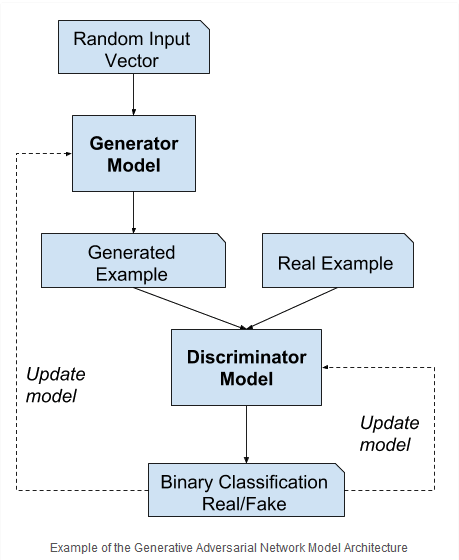
\includegraphics[width=0.6\textwidth]{GAN_Model}
    \caption{Funktionsprinzip eines \ac{GAN}}
    \label{Abb:basic}
    \end{figure}

    \noindent Die Abbildung zeigt die grundlegende Architektur eines \ac{GAN}, wie es auch schon in den Grundlagen zuvor erklärt wurde. Der Generator erhält als Eingabe einen zufälligen Vektor, der als Latent Space bezeichnet wird. Dieser Vektor wird als Eingabe in den Generator eingespeist und durchläuft eine Reihe von Schichten, die jeweils eine Reihe von Neuronen enthalten. Die letzte Schicht des Generators, die Ausgabeschicht, gibt einen Vektor aus, der die generierten Daten enthält. Der Diskriminator erhält schließlich als Eingabe entweder diesen oder einen aus echten Daten stammenden Vektor als Eingangswert. Dieser Vektor durchläuft anschließend einen ähnlichen Prozess, wie der Latent Space in Form des Diskriminators. Die letzte Schicht des Diskriminators gibt schließlich einen Vektor aus, der die Wahrscheinlichkeit angibt, ob die Eingabe aus echten oder generierten Daten besteht. Diese Wahrscheinlichkeit bietet in Form der \textit{Backpropagation} die Grundlage für das Training beider Modelle, allerdings auf zwei unterschiedliche Arten und Weisen. Sollte der Diskriminator nämlich falsch liegen und beispielsweise ein künstlich generiertes Bild als real anerkennen, so gilt dies für den Generator als Erfolg, für den Diskriminator allerdings als Fehlschlag. Dieses Verhältnis der beiden Modelle kann durch eine Funktion, die sogenannte \textit{Minimax-Verlustfunktion} \ref{eqn:Verlustfunktion} beschrieben werden.\\

    \begin{equation}
        \label{eqn:Verlustfunktion}
        L_{GAN}=\frac{1}{N_1}\sum_{i=1}^{N_1} \ln{D (\textbf{x}_i)} + \frac{1}{N_2}\sum_{j=1}^{N_2} \ln{(1-D (G (\textbf{z}_j)))}
        \end{equation}

    \noindent Der Diskriminator versucht dabei den oberen Term zu maximieren, indem korrekt zwischen echten und generierten Daten unterschieden wird. Der Generator hat allerdings die Fähigkeit den zwei Term zu beeinflussen, welchen er zu minimieren versucht. Diese Balance zwischen den beiden Modellen und ihren gegenseitigen Einflüssen, wird durch diesen Term gezeigt, welcher seinen Namen \textit{Minimax} exakt wegen diesem Hintergrund besitzt. 

    
    

\newpage